% !TEX root = ../thesis.tex
%
\chapter{Hintergrund}
\label{sec:concepts}
In diesem diesem Kapitel werden Grundlagen zu Wikidata und RDF\footnote{\url{https://www.w3.org/RDF/}} (Resource Description Framework), einem Standardformat zur Beschreibung von Informationen, erklärt. 

\section{Wikidata als strukturiertes Wiki}
Wikidata ist die gemeinsame Wissensdatenbank der Wikimedia Projekte.
Wie auch Wikipedia selbst baut Wikidata auf MediaWiki\footnote{\url{https://mediawiki.org}} auf, einer Software für das Betreiben von kollaborativen Wikis.
Im Gegensatz zu Wikipedia verwaltet Wikidata jedoch strukturierte Dokumente.
Die Erweiterungen für MediaWiki dazu stellt das Wikibase\footnote{\url{htts://wikiba.se}} Projekt bereit.

Alle Dokumente in Wikidata besitzen einen eindeutigen Identifier.
Dieser beginnt mit einem Großbuchstaben, der den Typ des Dokuments angibt, gefolgt von einer Zahl.
Aktuell kennt Wikidata drei Typen von Dokumenten: Items (Q), Properties (P) und Lexemes (L).
Lexemes wurden erst später hinzugefügt, so dass sie von dem in dieser Arbeit verwendeten Wikidata-Toolkit noch nicht vollständig unterstützt werden.
In dieser Arbeit werden Lexemes daher nicht genauer betrachtet.

Den Hauptbestandteil der Daten bilden jedoch die Items.
Ein Item repräsentiert ein bestimmtes Konzept, zu dem Fakten in Wikidata erfasst werden.
Der Aufbau eines Items ist beispielhaft anhand von \verb|Q42| (Douglas Adams) in \cref{fig:wd-datamodel} dargestellt.
Den ersten Teil bilden die Terme: \verb|label|, \verb|description| und \verb|aliases| dienen zur Beschreibung und Definition des Items.
Die Terme sind mehrsprachig: ein Item kann ein \verb|label| für jede der möglichen Sprachen haben.
Darauf folgen Statements, welche die Fakten zu diesem Item wiedergeben.
Zusätzlich kann jeder Item noch eine Reihe an Sitelinks besitzen. 
Diese verlinken auf andere Seiten des Wikimedia Projekts zum Thema des Items.
Die Sitelinks von \verb|Q42| verlinken zum Beispiel auf Artikel von Douglas Adams in den unterschiedlichen Sprachversionen von Wikipedia und in Wikiquote.

Die Fakten eines Items werden in Statements beschrieben.
Ein Statement besteht aus zwei Teilen: einem Claim, der eine bestimmte Aussage trifft, und einer Liste von Referenzen.
Da auch Statements ohne Referenzen erlaubt sind, kann die Liste der Referenzen auch leer sein.
Wikidata unterstützt drei Arten von Aussagen, genannt Snaks:
\begin{description}
\item[PropertyValue] die am meisten verwendete Art einer Aussage. Sie beschreibt den Fakt, dass eine bestimmte Eigenschaft (Property) einen gewissen Wert (Value) hat. Die Property bestimmt dabei den Typ der Value. Values können je nach Property andere Items oder skalare Werte (wie Zahlen, Zeichenketten, Koordinaten, Zeiten, usw.) sein.
\item[SomeValue] diese Art der Aussage wird verwendet, um auszudrücken, dass ein Wert für die Eigenschaft existiert der aber nicht bekannt ist. Zum Beispiel kann die Aussage ``es existiert ein Wert für den Todeszeitpunkt einer Person'' verwendet werden, falls eine Person gestorben ist, der Todeszeitpunkt aber nicht bekannt ist.
\item[NoValue] drückt aus, dass es für eine bestimmte Eigenschaft keinen Wert gibt. Wird verwendet, wenn das Fehlen einer Information keine Unvollständigkeit darstellt. Kann zum Beispiel für \verb|P200| (Zuflüsse) verwendet werden, wenn ein Gewässer keine Zuflüsse besitzt. 
\end{description}
Der Claim eines Statements besteht aus einem MainSnak, der die Hauptaussage darstellt, und zusätzlichen Qualifiern zur Verfeinerung der Aussage.
Eine Referenz ist auch einfach eine Liste von Snaks. 
Ein MainSnak zu Douglas Adams (Q42) ist zum Beispiel \verb|P69| (educated at) - \verb|Q691283| (St John's College).
Mit den Qualifier-Snaks wie \verb|P582| (end time) - \verb|1974| bildet dieser dann einen Claim.
Das Statement setzt sich dann aus diesem Claim und der Liste von Referenzen zusammen.
Alle Statements für die gleiche Property werden in einer Statement Group zusammengefasst.
Jedes Statement besitzt zusätzlich noch einen Rank (deprecrated, normal oder best) um die Priorität innerhalb der Statement Group auszudrücken.

Dieses Dokument-orientierte Datenmodell lässt sich einfach als JSON\footnote{\url{https://www.json.org}} (JavaScript Object Notation) repräsentieren.
Die vollständige Darstellung ist jedoch sehr umfangreich und ist deshalb aus Platzgründen hier nicht abgebildet.
Für ein Entity kann die JSON-Repräsentation einfach online abgerufen werden, für \verb|Q42| zum Beispiel unter folgender URL: \url{https://www.wikidata.org/wiki/Special:EntityData/Q42.json}.
Zusätzlich stellt Wikidata Exporte aller Dokumente als JSON bereit.

\begin{figure}
  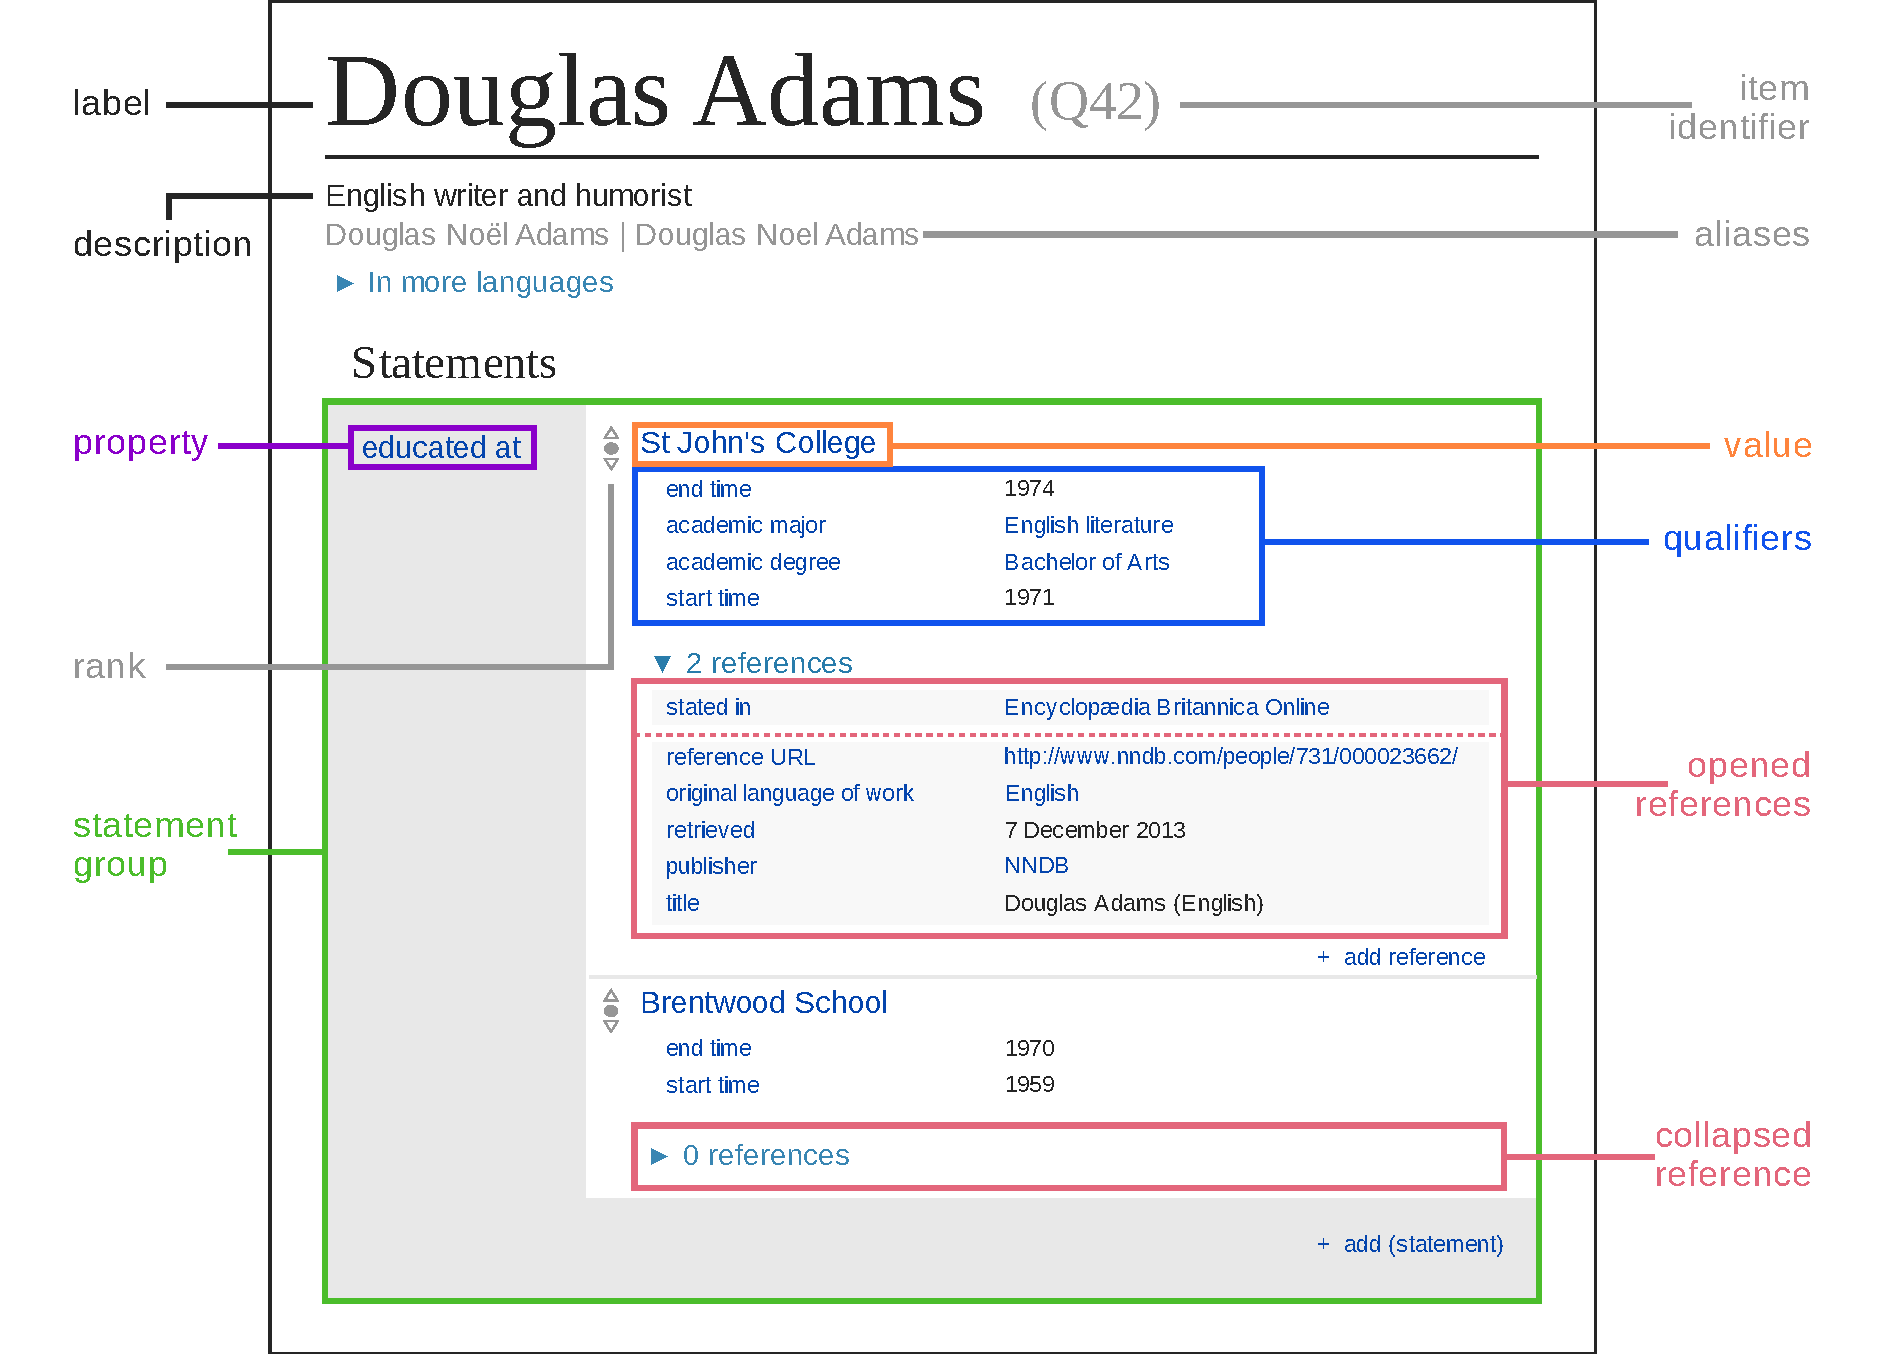
\includegraphics[width=\linewidth]{pics/Datamodel_in_Wikidata}
  \caption{Wikidata Item ``Q42''}
  \label{fig:wd-datamodel}
\end{figure}

\section{Wikidata als Linked Data}
Eine Besonderheit von Wikidata ist die starke Verlinkung der Daten untereinander.
Diese Verlinkung ermöglicht eine Art des Zugriffs, die sich von der dokumentbasierten Betrachtungsweise unterscheidet.
Fragestellungen wie ``Wer sind die Verwandten von Douglas Adams?'' oder ``Welche berühmten Personen sind in einem Staat geboren, der Mitglied der europäischen Union ist?'' betrachten die Beziehungen der Dokumente, und nicht allein den Inhalt einzelner Dokumente.

Das W3C hat für solche Graph-basierten Daten das Resource Description Framework (RDF) entwickelt.
In RDF werden als eindeutige Bezeichner Internationalized Resource Identifiers (IRIs)\footnote{https://www.ietf.org/rfc/rfc3987.txt} verwendet.
IRIs sind eine Erweiterung von URIs zur Unterstützung von internationalen Zeichensätzen.
In der Praxis werden für IRIs oft HTTP URLs verwendet, sodass Namenskonflikte zwischen unterschiedlichen Organisationen vermieden werden.
Außerdem können über HTTP weitere Informationen zu der entsprechenden Ressource bereitgestellt werden.

Das Kernelement von RDF bilden Tripel. Die drei Komponenten jedes Tripel sind:
\begin{description}
\item[Subjekt] eine IRI oder Blank Node
\item[Prädikat] eine IRI
\item[Objekt] eine IRI, Blank Node oder Literal
\end{description}
Blank Nodes sind lokale Bezeichner, die im Gegensatz zu IRIs nur innerhalb eines Dokuments eindeutig sein müssen.
Verschiedene RDF Dokumente können daher die selben Blank Node Bezeichner verwenden, ohne dass damit die selbe Resource beschrieben wird.

Literale in RDF sind Zeichenketten, die jedoch zusätzlich noch einen Datentypen oder einen Language Tag besitzen können.
Mit dem Datentyp kann die Interpretation der Zeichenkette genauer spezifiziert werden.
Auch Datentypen werden über IRIs referenziert.
Language Tags geben die Sprache der Zeichenkette als Language Code nach BCP47\footnote{\url{https://tools.ietf.org/html/bcp47}} an. In diesem Fall muss der Datentyp \url{http://www.w3.org/1999/02/22-rdf-syntax-ns#langString} sein.

RDF Dokumente sind eine Kollektion von Tripeln, wobei die Reihenfolge keine Rolle spielt.
Für die Serialisierung von RDF gibt es verschiedene Standards, ein einfacher und verbreiteter ist N-Triples\footnote{\url{https://www.w3.org/TR/n-triples/}}.
Die Syntax von N-Triples ist in folgendem Beispiel examplarisch dargestellt:
\begin{lstlisting}[language=SPARQL, breaklines=true]
<https://example.org> <http://schema.org/name> "Beispiel"@de .
<https://example.org> <http://schema.org/name> "Example"@en .
_:paper <https://example.org/about> <https://example.org> .
_:paper <https://example.org/popularity> "42"^^<http://www.w3.org/2001/XMLSchema#integer> .
\end{lstlisting}
Jede Zeile entspricht einem Tripel und wird mit einem Punkt abgeschlossen.
In N-Triples werden IRIs in \verb|<>| eingeschlossen und Blank Nodes durch das Prefix \verb|_:| markiert.
Literale sind von \verb|"| umgeben, mit \verb|@| bzw \verb|^^| können Language Tag und Datentyp angegeben werden.

In dieser Arbeit wird zur Übersichtlichkeit eine Erweiterung der Notation verwendet.
Dabei werden IRIs durch die Einführung von den in \cref{tab:rdf-prefixes} aufgeführten Prefixen vereinfacht.
Zum Beispiel wird \verb|<http://schema.org/name>| als \verb|schema:name| abgekürzt. 

\begin{table}
\begin{tabular}{l l}
\bfseries{Prefix} & \bfseries{URL} \\
rdf: & <http://www.w3.org/1999/02/22-rdf-syntax-ns\#> \\
xsd: & <http://www.w3.org/2001/XMLSchema\#> \\
% ontolex: & <http://www.w3.org/ns/lemon/ontolex\#> \\
% dct: & <http://purl.org/dc/terms/> \\
rdfs: & <http://www.w3.org/2000/01/rdf-schema\#> \\
owl: & <http://www.w3.org/2002/07/owl\#> \\
skos: & <http://www.w3.org/2004/02/skos/core\#> \\
schema: & <http://schema.org/> \\
% cc: & <http://creativecommons.org/ns\#> \\
geo: & <http://www.opengis.net/ont/geosparql\#> \\
prov: & <http://www.w3.org/ns/prov\#> \\
wikibase: & <http://wikiba.se/ontology\#> \\
wdata: & <http://www.wikidata.org/wiki/Special:EntityData/> \\
% bd: & <http://www.bigdata.com/rdf\#> \\
wd: & <http://www.wikidata.org/entity/> \\
wdt: & <http://www.wikidata.org/prop/direct/> \\
wdtn: & <http://www.wikidata.org/prop/direct-normalized/> \\
wds: & <http://www.wikidata.org/entity/statement/> \\
p: & <http://www.wikidata.org/prop/> \\
wdref: & <http://www.wikidata.org/reference/> \\
wdv: & <http://www.wikidata.org/value/> \\
ps: & <http://www.wikidata.org/prop/statement/> \\
psv: & <http://www.wikidata.org/prop/statement/value/> \\
psn: & <http://www.wikidata.org/prop/statement/value-normalized/> \\
pq: & <http://www.wikidata.org/prop/qualifier/> \\
pqv: & <http://www.wikidata.org/prop/qualifier/value/> \\
pqn: & <http://www.wikidata.org/prop/qualifier/value-normalized/> \\
pr: & <http://www.wikidata.org/prop/reference/> \\
prv: & <http://www.wikidata.org/prop/reference/value/> \\
prn: & <http://www.wikidata.org/prop/reference/value-normalized/> \\
wdno: & <http://www.wikidata.org/prop/novalue/>
\end{tabular}
\caption{Verwendete Prefixe. Diese werden auch vom Wikidata SPARQL Service vordefiniert.}
\end{table}

RDF kennt weder Referenzen noch Qualifier und kann im Gegensatz zu Wikidata auch nicht mehrere gleiche Tripel speichern.
Erxleben, Günther, Krötzsch, Mendez und Vrandečić haben 2014 beschrieben, wie trotzdem eine Darstellung als RDF möglich ist und auch ein System zur Erstellung regelmäßiger Exporte als RDF entwickelt \cite{wikidata-rdf-export}.
Nach dem Prinzip der Reifikation werden Statements, Referenzen und komplexe Werte nicht direkt als Tripel exportiert, sondern als eigene Ressourcen. 
Diese Ressourcen besitzen dann ein Tripel das zu dem Objekt des Statements verlinkt, aber auch zusätzlich Tripel für Qualifier und Referenzen.
Jedes Statement hat somit einen eindeutigen Namen, sodass auch zwei Statements mit dem selben Inhalt erfasst werden können.
\begin{figure}
  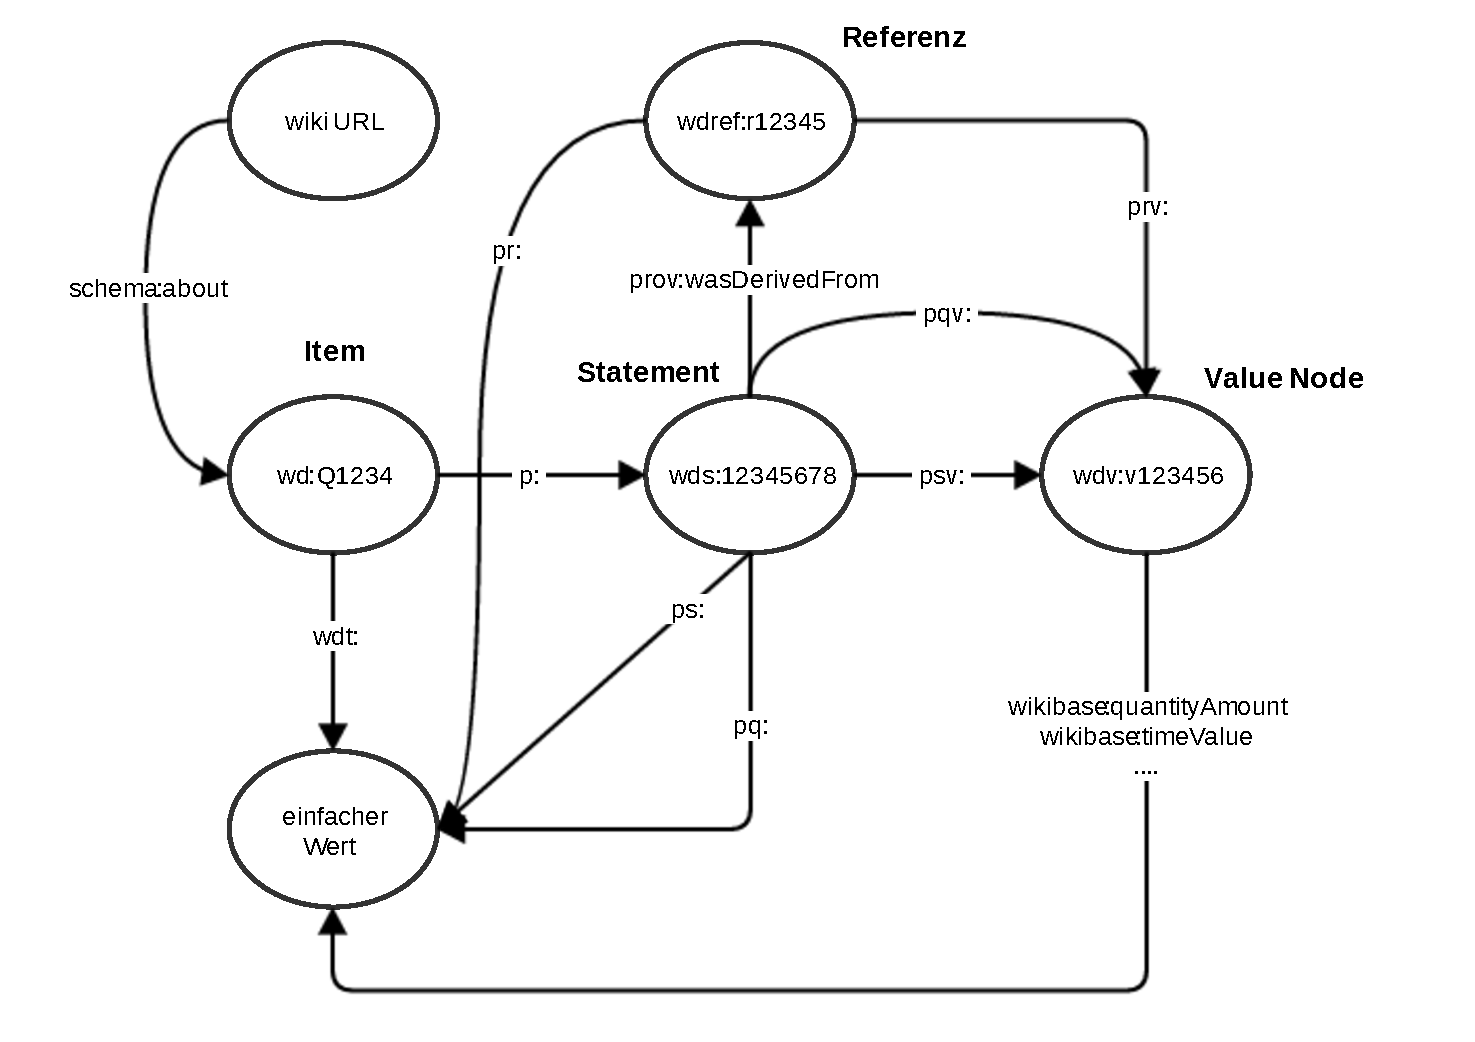
\includegraphics[width=\linewidth]{pics/Rdf_mapping}
  \caption{Mapping des Datenmodells auf RDF}
  \label{fig:rdf-mapping}
\end{figure}

Diese Übersetzung ist in \cref{fig:rdf-mapping} gezeigt.
Jeder Pfeil beschreibt dabei Prädikatprefix, welches dann für RDF-Tripel verwendet wird.
An dieses Präfix wird der Bezeichner der Property angehangen.
Hier ist ein Beispiel zur Verdeutlichung (gekürzt, die Informationen zu den Reference und Value Nodes sind nicht abgebildet):
\begin{lstlisting}[language=SPARQL]
wd:Q42 p:P26 wds:q42-xxxx .
wds:q42-xxxx rdf:type wikibase:Statement .
wds:q42-xxxx ps:P26 wd:Q14623681 .
wds:q42-xxxx pq:P580 "1991-11-25T00:00:00Z"^^xds:dateTime .
wds:q42-xxxx pqv:P580 wdv:c8ae0d38443d4671d3f893d7000a859e .
wds:q42-xxxx pq:P582 "2001-05-11T00:00:00Z"^^xsd:dateTime .
wds:q42-xxxx pqv:P582 wdv:1c30ade7914d072877b2db404a683d7c .
wds:q42-xxxx prov:wasDerivedFrom wdref:yyyyyyyy .
wd:Q42 wdt:P26 wd:Q14623681 .
\end{lstlisting}
Das Beispiel zeigt, wie die Property \verb|P26| (spouse) zuerst mit dem Prädikat \verb|p:P26| auf das Statement verlinkt.
Das Statement verlinkt dann über \verb|ps:P26| zum einfachen Wert der Property.
Mit \verb|pq:P580| (start time) bzw. \verb|pqv:P580| wird auf die einfache und komplexe Darstellung des Wertes für diesen Qualifier verlinkt.
Die komplexe Darstellung enthält noch weitere Informationen zu dem Datum, wie bspw. die Genauigkeit oder das verwendete Kalendermodell.

Eine spezielle Bedeutung hat der \verb|wdt:| Prefix.
Tripel mit diesen Prädikaten verlinken Items direkt mit den einfachen Werten.
Diese Tripel existieren allerding nur dann, wenn das zugehörige Statement vom Typ \verb|BestRank| hat.
Dieser Typ umfasst alle Statements, die den höchsten Rang für diese Property haben und nicht deprecrated sind.
Solche Statements und Tripel werden auch als ``truthy'' bezeichnet.
Die truthy Tripel sind sehr hilfreich, wenn man nicht an Qualifiern, Referenzen oder komplexeren Werten interessiert ist.
Für diesen Fall bieten sie eine einfachere Sicht auf die Daten, was besonders bei Abfragen die Komplexität reduziert.
